\chapter{Grundlagen}

\section{Maschinelles Lernen (Machine Learning)}

    Wenn man Maschinelles Lernen oder Künstliche Intelligenz hört, denkt die Mehrzahl an Roboter mit eigenem Bewusstsein und Denken wie in vielen Science Fiction Filmen dargestellt.
    Jedoch ist Maschinelles Lernen mittlerweile keine Zukunftstechnologie mehr.
    Bereits in den 60er Jahren gab es erste Versuche der Wissenschaft Künstliche Intelligenz zu erschaffen.
    Doch was ist Maschinelles Lernen wirklich? Und was bedeutet es für einen Computer zu lernen?
    \newline

    \noindent
    Dieses Kapitel beschäftigt sich mit diesen Fragen und gibt einen kurzen Überblick über heutige Verfahren von Maschinellem Lernen.

    \subsection{Künstliche Intelligenz}
    Bevor Maschinelles Lernen erklärt werden kann sollte Künstliche Intelligenz im allgemeinen geklärt werden.


    \subsection{Einführung}
    Nimmt man den Begriff Maschinelles Lernen wörtlich beschreibt er das Lernen einer Maschine, also die Fähigkeit einer Maschine inteligenter zu werden.
    Von Maschinellem Lernen spricht man, falls eine Maschine auf Basis von Erfahrung und Fakten "`ohne speziell programiert worden zu sein"'\cite[20]{HandsOnML}, neues Wissen oder neue Zusammenhänge generieren kann.
    Wenn eine Maschine nachdem sie etwas gelernt hat bei der Ausführung einer Aktivität besser geworden ist, hat die Maschine maschinel gelernt\cite[20]{HandsOnML}.
    Das reine auswendig lernen von Fakten, wie beispielsweise das abspeichern einer Wikipedia-Seite auf die lokale Festplatte eines Computers, ist kein Wissenserwerb.
    \newline

    \noindent
    Ein Beispiel für Maschinelles Lernen ist der Spamfilter bei Emails.
    Hier lernt ein Computer auf Basis von bisherigen Spammails neue Emails als Spam zu erkennen.
    \newline

    Der Einsatz von Maschinellem Lernen hat meist Vorteile gegenüber herkömmlichen Statistischen Methoden falls große Datenmengen ausgewertet werden müssen
    oder kein bekanntes Modell zur Problemlösung bekannt ist.
    Durch Maschinelles Lernen können Zusammenhänge erkannt werden, die durch andere statistische oder algorithmische Verfahren nicht erkannt oder abgebildet werden können.

    \subsection{Lernprozess} \label{Lernprozess}
    Grundlegend besteht Maschinelles Lernen aus einer Trainigsphase und einer Test- beziehungsweise Validierungsphase.
    Hierzu werden zunächst alle vorhandenen Daten in Trainings- sowie Testdaten meist im Verhältnis 80:20 eingeteilt.
    In der Trainigsphase wird auf Basis der Tringsdatendaten, wie zum Beispiel bisherige Emails eines Benutzers, ein Modell erstellt, welches dann in der Validierungsphase auf seine Genauigkeit und Validierungsgenauigkeit überprüft wird.
    Genauigkeit bedeutet, dass in der Validierungsphase alle Daten, welche auch im Traingsprozess verwendet wurden, von dem neuen Modell klassifiziert werden.\\
    Dieses Ergebnis wird dann mit der bekannten Klassifierung der Daten abgeglichen und eine Übereinstimmungswahrscheinichkeit errechnet, welche dann als Genauigkeit des Modells gilt.
    Um die Validierungsgenauigkeit zu berechnen wird derselbe Prozess auch mit den Testdaten durchgeführt.
    Die Validierungsgenauigkeit ist wichtig um herauszufinden ob das entstandene Netz die Trainingsdaten nur auswendig gelernt hat oder wirklich neues Wissen generiert hat.
    Dies ist der Fall, sobald während des Trainings die Validierungsgenauigkeit immer weiter sinkt, dann spricht man von Overfitting des Netzes.
    \newline

    \noindent
    Aus dem Ergebnis der Validierungsphase sowie der sonstigen Wissensbasis kann nun eine neue Trainsphase durchgeführt werden(vgl. \ref{fig:MLTrainigsprozess}).
    Dieser Prozess wird Epoche genannt und kann nun beliebig oft wiederholt werden und das Modell weiter verbessert werden.
    Das entstandene Modell stellt das neu generierte Wissen dar.

    % Schaubild zu testphasen hinzufügen
    \begin{figure}[H]
        \centering
        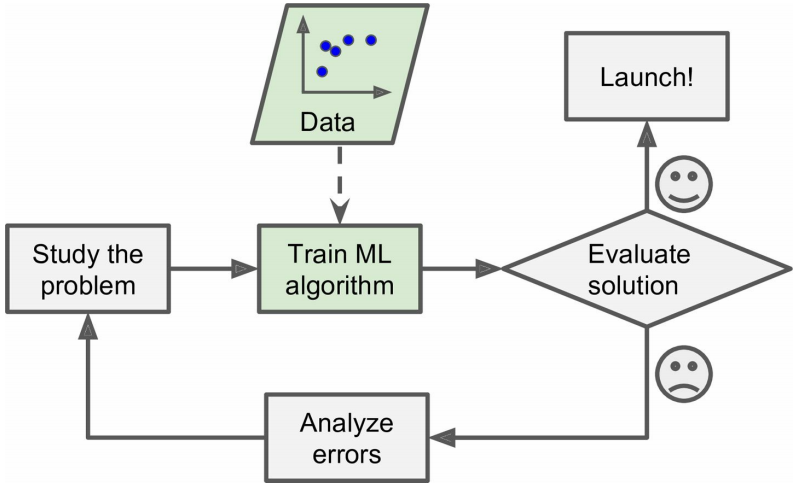
\includegraphics[width=\textwidth]{MLTrainigsphasen}
        \caption{Trainingsprozess (\cite[Figure 1-2]{HandsOnML})}
        \label{fig:MLTrainigsprozess}
    \end{figure}


    \section{Neuronale Netze}
    \cite[Vgl. im Folgenden]{EinfuehrunginNN,WissensbasierteSysteme}
    Neuronale Netze sind eine Form von Machinellem Lernen und die heute am meisten eingesetzte Technik für Bilderkennung, Spracherkennung oder Zeitreihenanalyse.
    
    \subsection{Aufbau}
    Ein künstliches neuronales Netz ist an das menschliche Gerhin angelehnt und soll dessen neuronales Netz sowie dessen Verhalten abbilden. 
    Dementsprechend besteht ein solches Netz aus mehren Neuronen und Schichten von Neuronen welche über Synapsen miteinander verbunden sind.


    \subsubsection{Neuronen}
    Neuronen bestehen aus Eingängen, auch Dendriten gennant, welche durch eine Eingangsfunktion, eine Aktivierungsfunktionen sowie eine Ausgabefunktion geleitet werden.
    Die Ausgabe eines Neurons besteht daraus dass dieses je nach Eingabe und Art entweder angereg("gefeuert") wird oder nicht.
    
    \begin{figure}[H]
        \centering
        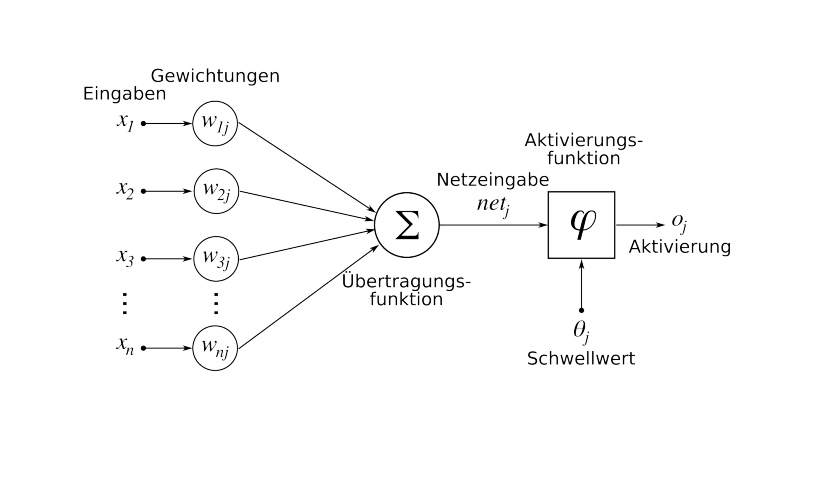
\includegraphics[width=\textwidth]{AufbauNN}
        \caption{Aufbau eines Neurons}
        \label{fig:AufbauNN}
    \end{figure}
    
    \noindent
    Die Eingangsfunktion berechnet aus den verschiedenen Eingängen den effektiven Eingang welcher dann weiter von der Aktivierungsfunktion verarbeitet wird.
    Diese effektive Eingabe ist dann die Netzeingabe in das Neuron.
    Meist wird die Netzaktivität \(net\) einfach als Summe aller Eingänge \(x\) und deren Gewichtungen \(w\) errechnet:
    \begin{equation}
        net = \sum_{i=0}^N x_i w_i
    \end{equation}
    \newline

    \noindent
    Die Aktivierungsfunktion dient zur eigentlichen Auswertung der Eingabe bzw. Netzaktivität.
    Die Aktivierungsfunktionen erzeugt ein Aktiverungspotential welches von der Ausgangsfunktion ausgewertet wird.
    \newline
    
    \noindent
    Die Ausgangsfunktion entscheidet schlussendlich ob das Neuron angeregt wird oder nicht.
    Hierzu wird geprüft ob das Aktivierungspotential der Aktivierungsfunktion einen bestimmten Schwellenwert übersteigt.
    Dieser Schwellenwert wird mithilde einer Schwellenwertfunktion errechnet. 
    Die Schwellenwertfunktion muss monoton wachsend sein, kann jedoch verschiedene Formen annehmen. 
    Sie kann linear Verlaufen wie es beim Perzeptron der Fall ist, nicht-linear oder eine Sprungfunktion sein. 
    Durch eine nciht-lineare Funktion wie die Sigmoid-Funktion lassen sich mächtigere neuronale Netze entwickeln weshalb heuzutage meist eine solche zum Einsatz kommt.


    \subsubsection{Topologie}
    Bei einem neuronalen Netz sind dessen Neuronen über Synapsen, welche bestimmte Kantengewichte bzw. Biases haben, verbunden.
    Durch verschiedene Kantengewichte können Eingänge oder bestimmte Features priorisiert werden. 
    Dies bedeutet, dass Eingänge welche größeren Einfluss auf das erwartetete Ergebnis haben, höher gewichtet werden können und somit stärker in das Ergebnis mit einbezogen werden.
    \newline

    \noindent
    Durch verschiedene Verbindungen zwischen Neuronen ergeben sich verschiedene Topologien von Netzen:
    \begin{description}
        \item[Vorwärts-verkettete Netze], auch feed-forword Netze genannt, bestehen aus verschiedenen Neuronen-Schichten(hidden layers), welche nur mit der nächst höheren Schicht verbunden sind. Somit verlaufen die Daten nur in eine Richtung, vom Eingang zum Ausgang.
        \item[Rekurrente Netze] können auch aus mehreren Neuronen-Schichten bestehen wobei hier auch verbindungen in tiefere Schichten möglich sind. Dies bedeutet, dass auch Ergebnisse von vorherigen Durchläufen des Netztes als Eingang mit einbezogen werden können.
        \item[Voll-vernetzte Netze] sind neuronale Netze, bei denen alle Neuronen mit allen anderen Neuronen vernetzt sind. Wobei hierbei keine wirkliche Struktur erkennbar ist und ein sehr großer Rechenaufwand besteht.
    \end{description}

    \begin{figure}[H]
        \centering
        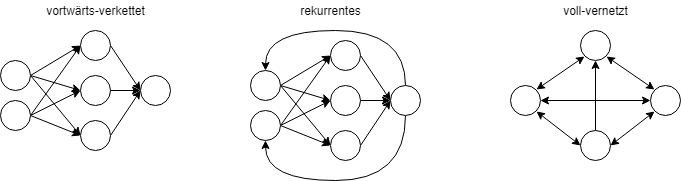
\includegraphics[width=\textwidth]{NetzTopologien}
        \caption{Netztopologien}
        \label{fig:NetzTopologien}
    \end{figure}


    \subsubsection{Lernen}
    Bei neuronalen Netzen ist das vorhandene Wissen durch die Kantengewichte repräsentiert.
    Daraus folgt, dass verschiedene Klassifikationen von neuronalen Netzen, mit derselben Topologie, sich nur von den Kantengewichten abhängt.
    Dementsprechend lernt ein neuronales Netz durch das sequentielle Anpassen der Gewichte.
    Dazu gibt es verschiedene Verfahren wie diese Gewichte angepasst werden können.
    \newline

    \noindent
    Beim \textbf{Backpropagation Lernen} werden in der Trainigsphase die Ergebnissen eines Durchlaufs mit den erwartetten Ergebnissen verglichen und der Ausgabefehler berechnet.
    Mithilfe dieses Fehlers wird nun Schichtweise versucht den Fehler auf einzelene Neuronen bzw. Gewichte bis hin zur Eingabeschicht zurückzuführen.
    Danach werden nun bei verschiedenen Neuronen Änderungen der Gewichte durchgeführt um den Fehler der Ausgabefehlerunktion zu minimieren.
    Hierbei wird für jedes Gewicht mithilfe verschiedener Gradientenverfahren eine Änderung berechnet.
    \newline

    \noindent
    Beim \textbf{Batch Lernen} wird anders als beim Backpropagation Lernen nciht nach jeden Durchlauf des Netztes die Gewichte angepasst sondern erst nachdem das Trainingsset komplett durchlaufen wurde.
    Dies führt zu weniger Genauigkeit das nicht auf spezielle Eigenschaften einzelener Einträge eingengangen.
    Jedoch Ist dieses Verfahren sehr viel weniger Rechenaufwand und es können mehr Trainingsdaten in gleicher Zeit einbezogen werden.
    
    \subsubsection{Perzeptron}
    Ein sehr einfaches neuronales Netz ist das Perzeptron, welches 1958 von Frank Rosenblatt entwickelt wurde.
    Das Perzeptron besteht aus zwei Eingabeparametern, welche in ein Neuron gegeben werden und von diesem mithilfe der Kantengewichte und der Aktivierungsfunktion eine Ausgabe liefert.

    Ein Beispiel ist die Abbildung des boolschen "`Und"'-Operators welche wie in Abbildung \ref{fig:PerzeptronAND} mit einem Neuron dargestellt werden kann.
    Jedoch können mit einem Neuron nur sehr einfache Funktionen abgebildet werden. 
    Komplexere Funktionen können über mehrere Neuronen bzw. mehrere Schichten von Neuronen abgebildet werden.

    \begin{figure}[H]
        \centering
        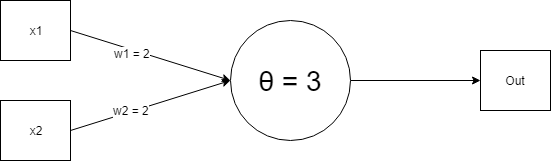
\includegraphics[width=\textwidth]{Perzeptron}
        \caption{UND-Operator als Perzeptron}
        \label{fig:PerzeptronAND}
    \end{figure}

    \begin{table}[H]
        \centering
        \begin{tabular}{|l|l|l|l|}
            \hline
            x1 & x2 & \( (x_1 * w_1) + (x_2 * w_2) \) & out \\
            \hline
            0 & 0 & \( (0 * 2) + (0 * 2) = 0 < 3 \) & 0 \\
            \hline
            0 & 1 & \( (0 * 2) + (1 * 2) = 2 < 3 \) & 0 \\
            \hline
            1 & 0 & \( (1 * 2) + (0 * 2) = 2 < 3 \) & 0 \\
            \hline
            1 & 1 & \( (1 * 2) + (1 * 2) = 4 < 3 \) & 1 \\
            \hline
        \end{tabular}
        \caption{Wahrheitstabelle des Perzeptron}
        \label{tabl:Perzeptron}
    \end{table}

    \subsection{CNN - Convolutional Neural Network}
    \subsection{RNN - Recurrent Neural Network}



\section{Physikalische Grundlagen zur Netzaktivität} \label{physikalischeGrundlagen}

\section{Erhebung der Messdaten} \label{Messdaten}

    Um aussagekräftige Analysen und Klassifikationen über ein Stromnetz bzw. die Geräte in einem Stromnetz mit Maschinellem Lernen machen zu können, werden viele Trainings- und Testdaten benötigt.
    Die Daten bestehen aus verschiedenen physikalische Größen, die zu einem bestimmten Zeitpunkt in einem Stromnetz auftreten.
    Zu diesen Größen gehört die allgemeine Netzspannung, die Netzfrequenz sowie sieben harmonischen Oberwellen (vgl. \ref{physikalischeGrundlagen}).
    Um einen allgemeinen Überblick über den Verlauf der Netzaktivität zu erhalten sowie verschiedene Zeiten und Geräte vergleichen zu können, müssen Daten über lange Zeiträume erhoben werden.\\
    \newline
    Zur Erhebung der Werte zur Netzaktivität wurde ein WeSense-Messgerät\footnote{http://www.wesense-app.com/home-en/} verwendet.
    Dieses Gerät misst alle benötigten Werte und sendet diese über einen MQTT-Broker\footnote{Message Queuing Telemetry Transport} an einen Service von WeSense, welcher dann die Daten aufbereitet und in einer MSSQL Datenbank abspeichert.
    Die Werte werden sekündlich gemessen und in die Datenbank gespeichert, weshalb zunächst in eine row-based Datenbank gespeichert wird und später dann die Daten in eine column-based Datenbank zur schnellen Abfrage überführt werden.
    \newline

    \begin{figure}[h]
        \centering
        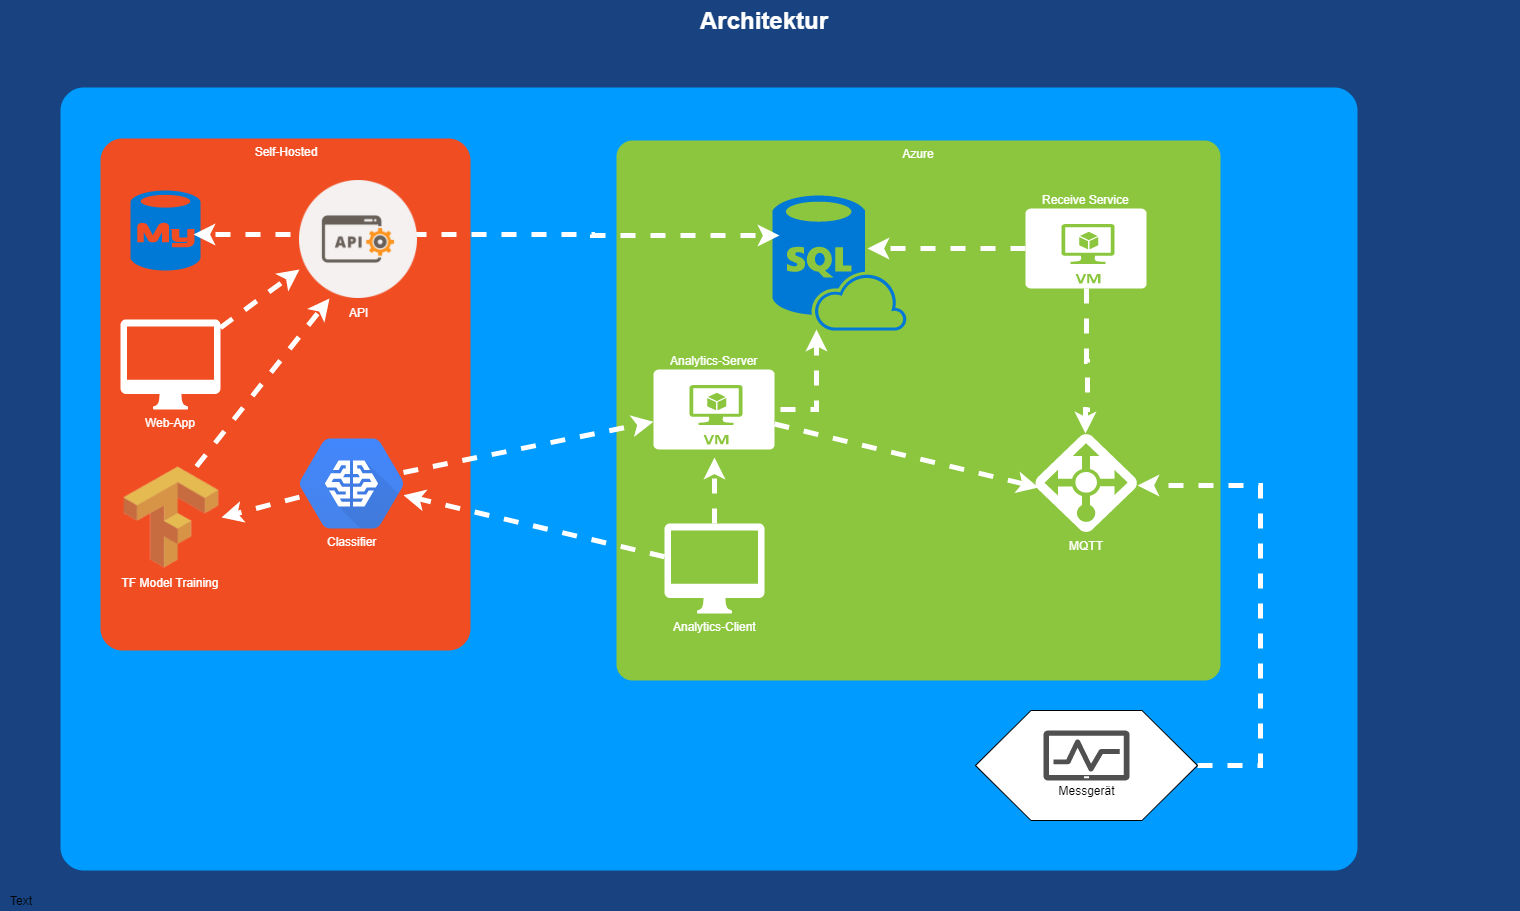
\includegraphics[width=1.0\textwidth]{Architecture}
        \caption{Complete Architecture}
        \label{fig:Architecture}
    \end{figure}

    \subsection{Klassifikation der Messdaten}\label{KlassifikationDerMessdaten}

        Durch die oben beschriebene Erhebung sind die physikalischen Werte zu bestimmten Zeitpunkten bestimmt worden.
        Zusätzlich wird nun zur Identifikation der Geräte sowie zum Maschinellen Lernen, genau definierte Zeiträume benötigt in denen bestimmte Geräte aktiv waren.
        Dies bedeutet, dass jedem Zeitpunkt ein oder mehrere Geräte zugewiesen werden. \\
        \newline
        Um diese gelabelten Daten zu erheben gibt es verschiedene Möglichkeiten.
        Die Daten können entweder durch eine Person, welche Zeiten zu denen sicher Geräte aktiv waren manuell erfasst, oder durch eine Maschine automatisch erhoben werden.
        Jedoch wird zur automatischen Erhebung ein weiteres Gerät benötigt, welches zwischen dem zu messenden Gerät und dem Stromnetz zwischengeschalten wird und sobald Strom fließt Daten erfasst.
        Somit werden die manuell durch eine Person erfasst.\\
        \newline
        Hierzu wurde eine progressiv Web-App(vgl. Abbildung \ref{fig:WebApp1}) mit einer einfachen MySQL-Datenbank erstellt, mit der die Daten sehr einfach erfasst und abgespeichert werden können.

        \begin{figure}[h]
            \centering
            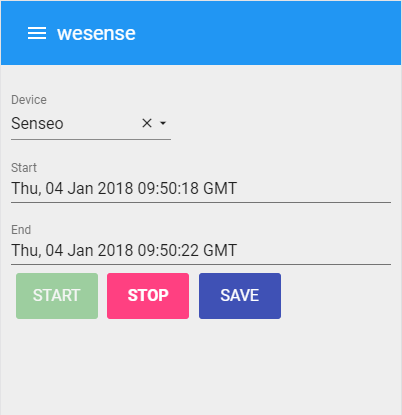
\includegraphics[width=0.5\textwidth]{WesenseConveyWebApp}
            \caption{Screenshot der progressive Web-App}
            \label{fig:WebApp1}
        \end{figure}

\section{Visualisierung}\label{VisualisierungWebApp}

        Zusätzlich zur manuellen Erhebung der Daten wurden zur besseren Analyse der Daten verschiedene Visualisierungsmöglichkeiten implementiert.
        Zum einen können die verschiedenen Physikalischen Größen eines gelabelten Gerätes zu einem bestimmten Zeitpunkt miteinander verglichen werden.
        Außerdem können bestimmte Größen zu verschiedenen gelabelten Zeiträumen eines Gerätes verglichen und analysiert werden.
        Durch diese Visualisierung können sehr gut und genau Gemeinsamkeiten in verschiedenen Größen oder Zeiten erkannt werden.\\
        \newline
        Es werden verschiedene Diagramme sowie Normalisierungen der Daten zur Analyse bereitgestellt.
        Es besteht die Möglichkeit die Daten in einem Liniendiagramm sekündlich oder in frei wählbaren zusammengefassten Datenpunkten, sogennannten Klassen, anzuzeigen.
        Des weiteren können Histogramme mit verschiedenen Klassen gewählt werden.

        \begin{figure}[h]
            \centering
            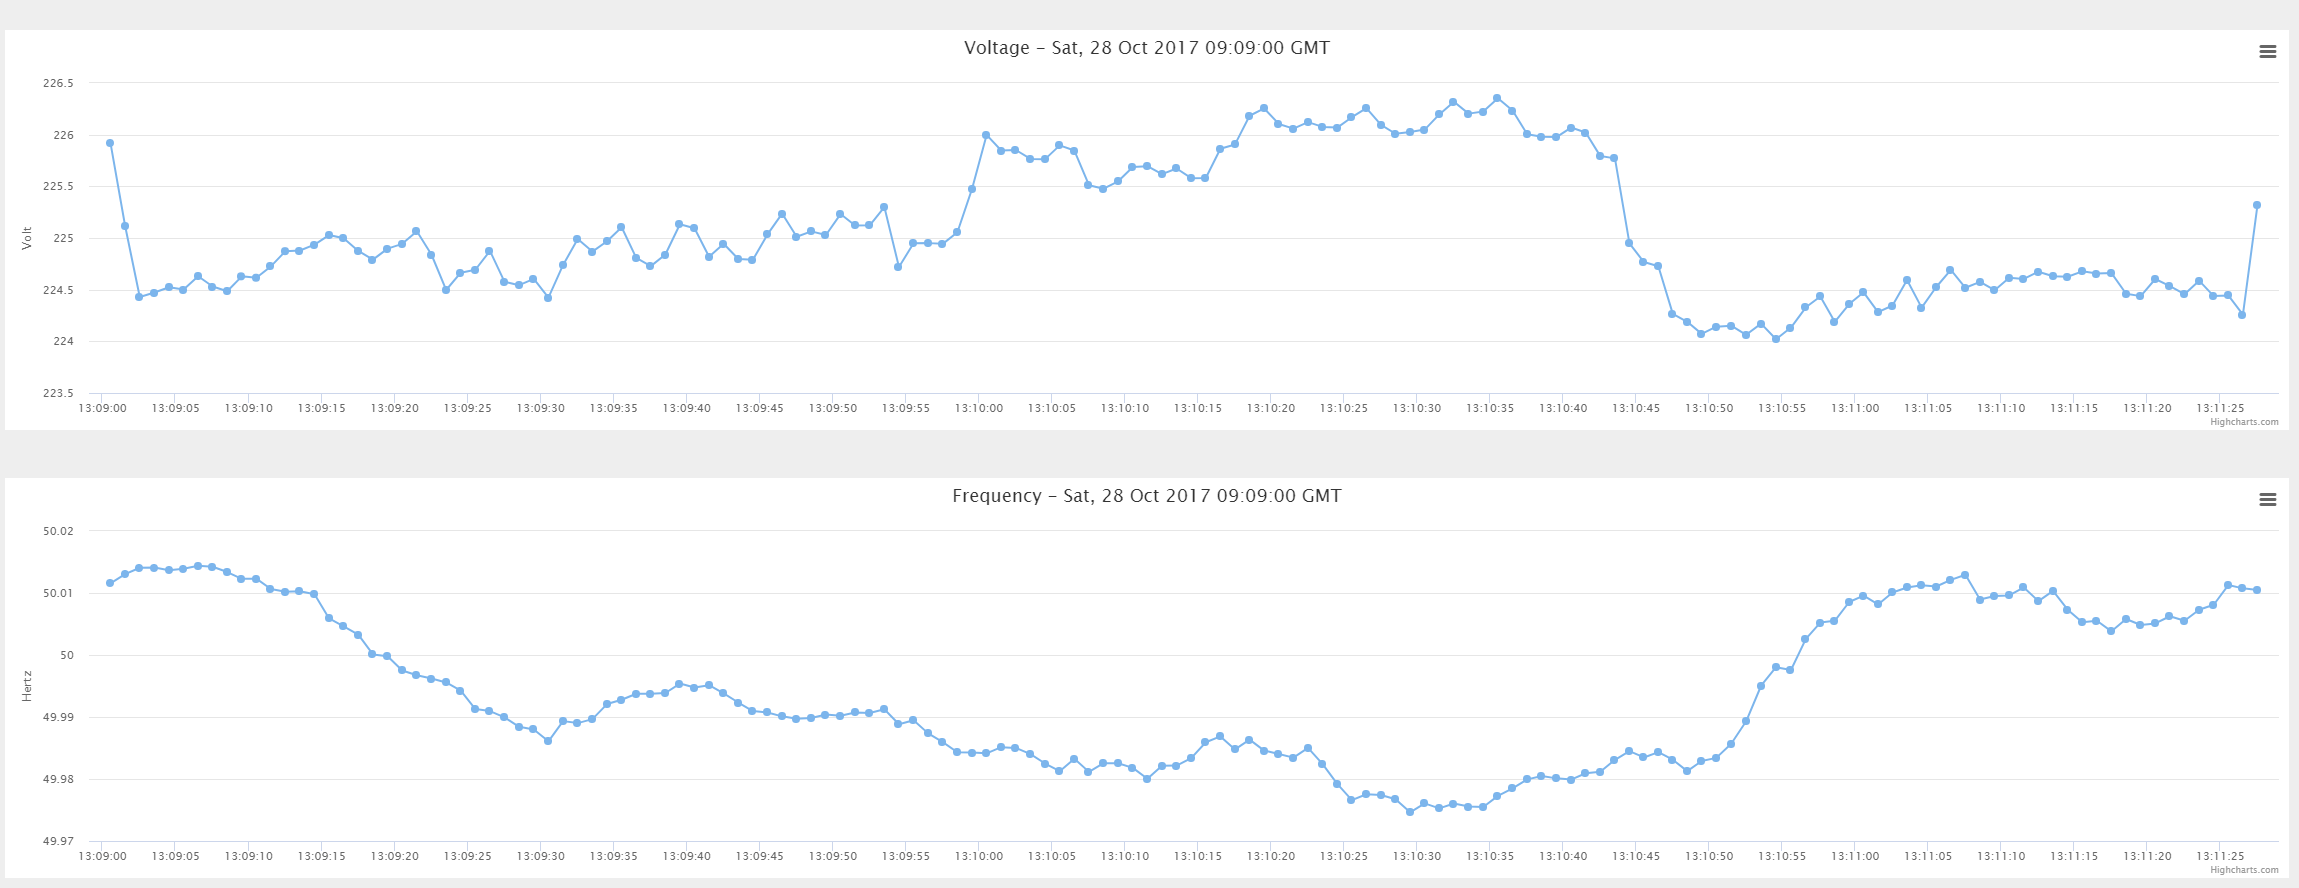
\includegraphics[width=0.75\textwidth]{WesenseConveylineChart}
            \caption{Screenshot eines gelabelten Zeitraumes aus der Web-App}
            \label{fig:WebApp2}
        \end{figure}
